\documentclass{cys}

\usepackage[utf8]{inputenc}

%\usepackage[english]{babel}
%\usepackage[spanish,mexico,es-tabla]{babel}
\usepackage[russian,english]{babel}  % If you use other languages, use Babel package.


\usepackage{graphicx}

\usepackage{epstopdf} % Avoid using plain Latex, use PDFLATEX

\addto\captionsenglish{%
  \renewcommand{\figurename}{Fig.}%
  \renewcommand{\abstractname}{Abstract.} 
%  \renewcommand{\keywordsname}{Keywords: } 
}

\addto\captionsspanish{%
  \renewcommand{\figurename}{Fig.}%
  \renewcommand{\abstractname}{Resumen.} 
%  \renewcommand{\keywordsname}{Palabras clave: } 
}


\title{A Container-Based Cloud Implementation of a Multi-Swarm PSO for Fuzzy Controller Optimization}

\author{Alejandra Mancilla$^1$, Mario García-Valdez$^1$, Oscar Castillo$^1$, Juan J. Merelo Guerv\'os$^2$}

\affil{ 
$^1$  Tijuana Institute of Technology / Tecnol\'ogico Nacional de M\'exico,   \authorcr   % Do not us full postal address!
Tijuana, Mexico

\authorcr \authorcr
$^2$  University of Granada, Department of Computer Engineering, Automatics and Robotics, \authorcr
Granada, Spain            
\authorcr  \authorcr
\{alejandra.mancilla,mario\}@tectijuana.edu.mx, ocastillo@tectijuana.mx, jmerelo@ugr.es
\authorcr  \authorcr
}


\begin{document}

\maketitle

\renewcommand{\tablename}{Table}

\begin{abstract}

The adoption of cloud-native technologies for distributed computing presents a
set of unique challenges. It's important to consider the cloud provider features
to achieve scalability, fault-tolerance, reproducibility, and cost-effectiveness
while maintaining intended functionality. This paper introduces a
container-based implementation of a cloud-native multi-population PSO on
Amazon's Elastic Container Service and evaluates its to solution and performance and
scalability. The study examines the impact of design parameters, such as
the number of swarms and the number of worker containers implementing isolated
PSO algorithms. Furthermore, the paper demonstrates that the proposed solution
is offering a robust alternative for both local and cloud environments. The
results underscore the benefits of containerization for cloud-based bioinspired
computing.

\end{abstract}

\begin{keywords} 
Cloud Computing, Multi-Swarm Optimization, Fuzzy Control
\end{keywords} 

\begin{figure*}[ht]
\centering
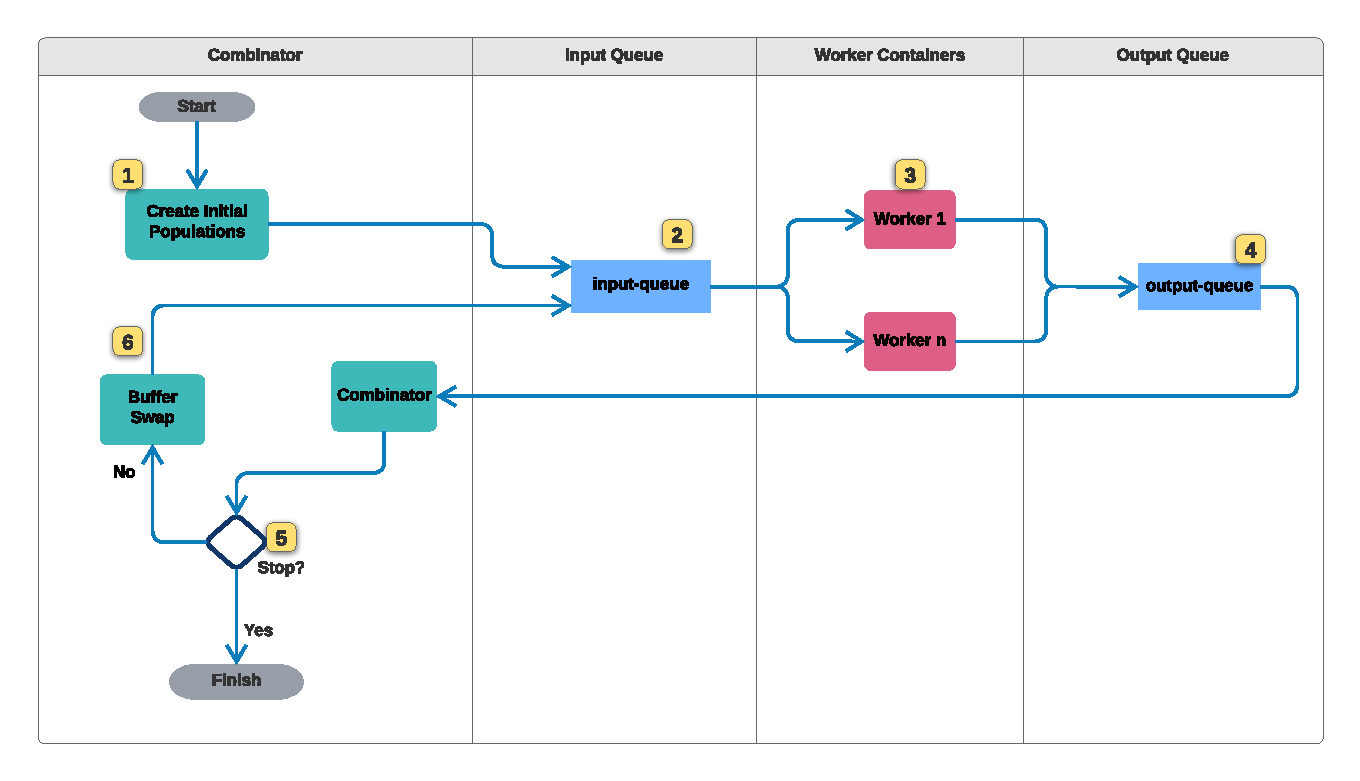
\includegraphics[width=\textwidth]{KafkEO}
\caption{Container-based architecture proposed by García-Valdez and Merelo \cite{valdez2021container} 
in which multiple swarms are created and
added to an \texttt{input-queue}, multiple workers then evolve these swarms, and finally,
they migrate in the \texttt{combinator} process. This cycle is repeated several times.
The dynamic adaptation of \texttt{C1} and \texttt{C2} is executed each time a swarm reaches the
\texttt{combinator}.}
\label{fig:KafkEO}
\end{figure*}

\section{Introduction}
\label{sec:introduction}

Cloud computing is becoming a standard way of running computer science experiments.  
This shift is largely attributed to its cost-effective, pay-as-you-go model, 
eliminating the hefty upfront investment and ongoing management expenses associated 
with local computing infrastructures. Furthermore, cloud computing simplifies defining
the infrastructure within the code itself, greatly enhancing the reproducibility 
of scientific computing results. A basic example of the benefits of having easily reproducible code is the rise of web-based 
interactive computing platforms such as the Jupyter Notebook project \cite{kluyver2016jupyter} 
or Google's Colaboratory \cite{carneiro2018performance} platforms.
When executing the interactive code, in these platforms, we can easily choose to scale the 
execution environment, using computing resources that greatly exceed what we have in 
our personal computers. This capability is a key advantage, enabling more complex and 
resource-intensive operations that go beyond the limitations of our local hardware.
A cloud-native implementation of a computational experiment also
has the capability of scaling from local execution to a wide range of execution options 
via cloud computing services like Amazon's AWS or Microsoft Azure. 
Cloud computing has evolved from hosting monolithic applications on virtual 
machines executing on remote data centers to other architectures. 
Presently, prevailing design patterns in cloud computing adhere to the principles of  
microservices \cite{microservices} and serverless \cite{varghese2018next}.
Microservices architecture \cite{malawski2017serverless} emphasizes breaking down
applications into smaller, loosely-coupled components, fostering flexibility and 
scalability. On the other hand, serverless computing further refines this paradigm by abstracting away 
infrastructure concerns, enabling developers to focus solely on code execution and 
minimizing resource allocation to match application demands dynamically. 
The combined use of these design patterns enhances the efficiency and adaptability of
computational experiments in cloud-native environments.

{\em Cloud-native applications} bring new methodologies and
techniques \cite{Baldini2016287}. To better exploit the capabilities of the cloud
infrastructure, applications are implemented as reactive systems \cite{boner2014reactive}
that are generally more scalable, flexible, and fault-tolerant. A reactive system can be
implemented as a loosely coupled collection of microservices.

These components are easily implemented and deployed to cloud environments, where
processing nodes can be defined and deployed using scripts, and scalable message 
queue services are provided to easily send and receive events. Additionally, 
scalability in such systems is achieved through the automatic provisioning of 
additional computing nodes as demand increases or in response to node failures, 
ensuring consistent performance and reliability.

\begin{figure*}[ht]
\centering
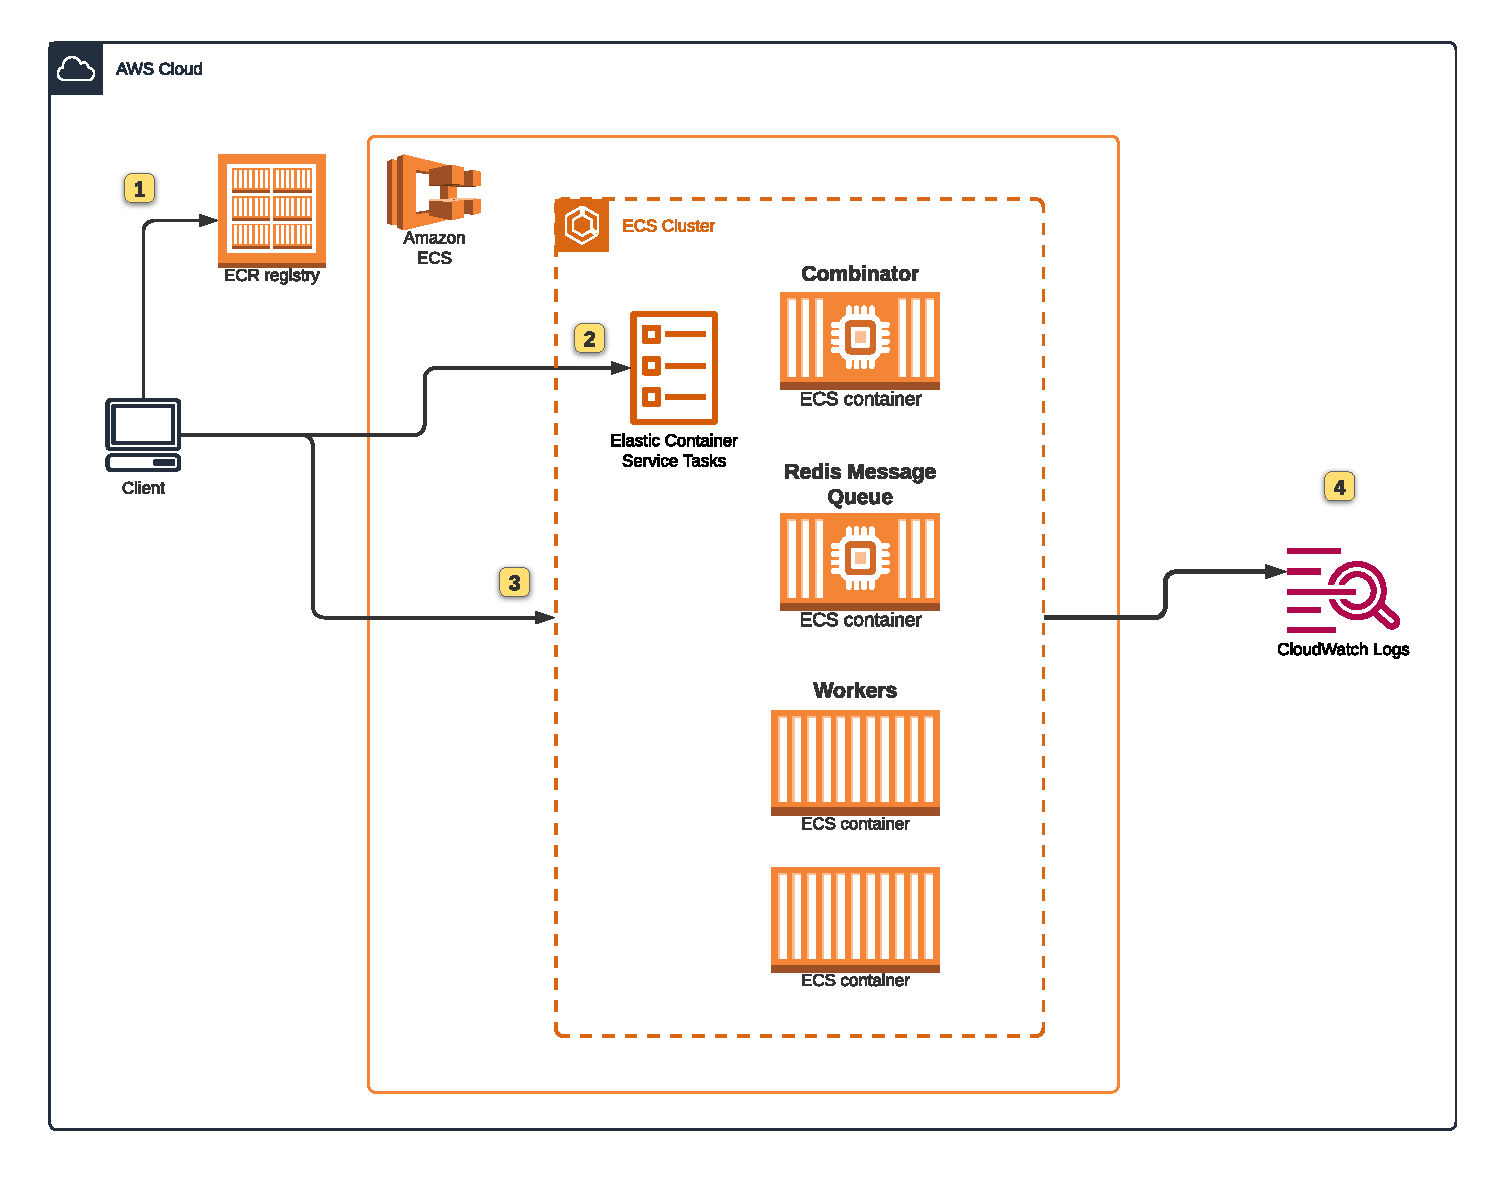
\includegraphics[width=\textwidth]{aws-deployment}
\caption{Implementation using AWS cloud technologies}
\label{fig:aws-deployment}
\end{figure*}

Microservices are typically executed within isolated runtime environments called
containers. These containers do more than just provide a runtime environment; 
they encapsulate all the necessary components required for the microservice to 
function autonomously. 
This includes software libraries, binaries, and configuration files. Essentially, 
containers package everything that a node needs to operate.
The strength of a containerized application lies in its ease of operation on automation platforms. 
These platforms are capable of taking containerized microservice-based
applications from a local computer to be deployed in a cloud or an ephemeral 
infrastructure \cite{gilbert2018cloud,kratzke2017understanding}. 

In our previous research \cite{merelo2019scaling}, we highlighted that a 
reactive architecture is well-suited for implementing population-based metaheuristics if they require 
extensive computational resources. Building on this foundation, the current work details the 
deployment process of a reactive, container-based, multi-swarm PSO algorithm specifically designed for deployment in Amazon's AWS.
The optimization problem tackled in this work is presented in \cite{mancilla2021optimization} 
and consists of tuning the membership functions of a fuzzy controller. This 
optimization problem is computationally intensive, primarily because it requires 
evaluating the fitness of all potential solutions.
This evaluation process involves running multiple simulations for each candidate 
solution, as further explored in \cite{mancilla2022tracking,mancilla2022optimal}. 
Despite the computational demands of this optimization problem, the independent 
nature of solution evaluation in evolutionary algorithms allows for the efficient parallelization of work.
In the literature, we found only a few works \cite{cortes2014optimal,oh2009design,ciurea2013determining}
attempting to distribute fuzzy controller's optimization; however, these works
have not fully leveraged the advancements in cloud-native technologies.

This gap presents an opportunity to explore how modern cloud-native solutions can 
enhance population-based optimization. This examination focuses on the intricacies of 
deploying such an algorithm within a cloud environment, leveraging the scalability and 
flexibility of AWS services. The use of containerization, a key feature of this deployment, 
offers the benefit, of having environment consistency and ease of scalability. This 
approach aligns with the principles of reactive systems, ensuring that the deployed 
algorithm is efficient in resource usage and robust and adaptable to varying computational loads.

In summary, our approach addresses a fuzzy control problem through the application
of a cloud-native distributed Particle Swarm Optimization (PSO) algorithm, characterized 
by its minimal set of tunable parameters. We emphasize the significance of our design 
choices and elucidate the deployment process leveraging various cloud technologies 
provided by Amazon's AWS.

This paper is dedicated to a cost analysis, comparing multiple 
configurations of both local and cloud deployments. By scrutinizing the associated 
costs, we aim to provide insights into the economic considerations associated with 
implementing our proposed solution in different computing environments.


We organized the paper as follows: First, Section \ref{sec:relatedWork} presents state of the art relevant to our work. 
In Section \ref{sec:aws-deployment}, we present the proposed method and the container-based
cloud deployment in Section \ref{sec:use_case} we present the use case and experimental setup to assess 
deployment options, concerning time-to-solution performance, discussing  the results in Section \ref{sec:results}. 
Finally, we offer the conclusions and suggestions for future work in Section \ref{sec:conclusionAndFutureWork}.

\begin{figure}[ht]
\centering
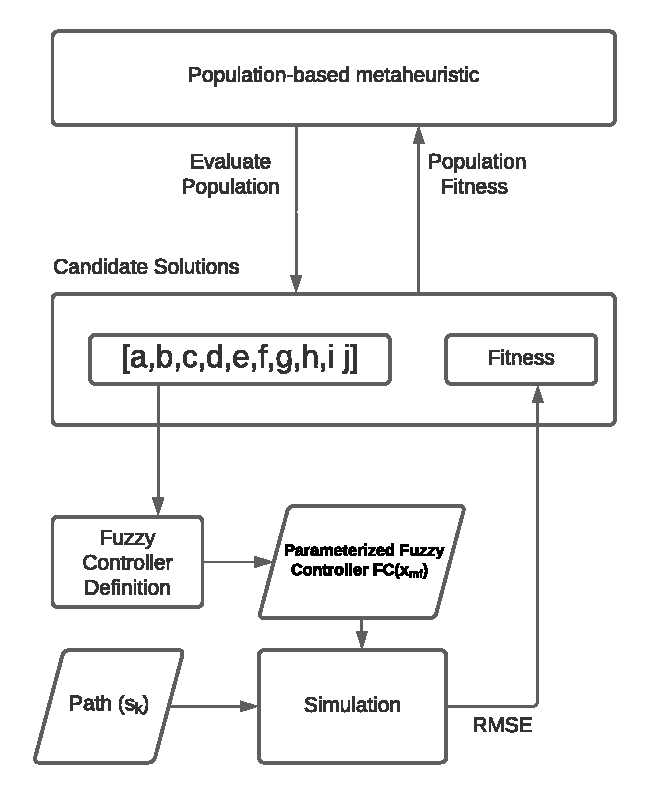
\includegraphics[width=0.4\textwidth]{fisopt}
\caption{Fuzzy Controller Problem \cite{mancilla2022tracking}.}
\label{fig:Eval}
\end{figure}


\section{Related Work}
\label{sec:relatedWork}
One of the primary features that make containers interesting is their
ephemeral nature: fast startup and tear-down time make them usable for
machine-independent and cloud deployment of simple, ephemeral, and
sometimes stateless functions. 
Furthermore, containerization, facilitated by orchestration engines 
such as Docker Swarm or Kubernetes, as well as non-self-scaling 
specifications like {\tt docker-compose}, enables the explicit 
definition of relationships between different components or services 
within an application. This orchestration capability empowers 
developers to articulate the intricate interdependencies within their applications.

The realization of Docker-based architectures \cite{kratzke2017understanding} has
given rise to a set of patterns that collectively delineate the landscape of
cloud-native application development. 

\begin{table}[ht]
\small
\caption{Cost AWS} \label{tab:costos}
\begin{tabular}{p{3.4cm}  p{2cm}  p{1.5cm} }
Service                           & Price         & Free tier \\
\hline 
\multicolumn{3}{c}{\textbf{Elastic Container Registry}  }              \\
\hline
Storage                           & \$0.10 per GB & 50 GB     \\
All data transfer IN              & \$0.00 per GB &           \\
Data Transfer OUT                 &               &           \\
Next 9.999 TB / month             & \$0.09 per GB &           \\
\hline
\multicolumn{3}{c} {\textbf{AWS Fargate}  }                           \\
\hline
per vCPU per hour                 & \$0.040480    &           \\
per GB per hour                   & \$0.004445    &           \\
Fargate Ephemeral Storage GB per hour   &  \$0.000111   &  20 GB \\
\hline
\multicolumn{3}{c}{\textbf{Amazon Cloud Watch} }                       \\
\hline
Collect (Data Ingestion)          &               &           \\
    Standard              & \$0.50 per GB & 0 to 5 GB  \\
    Infrequent Access     & \$0.25 per GB & 0 to 5 GB \\ \hline
\end{tabular}
\end{table}

\begin{table*}[ht]
\centering
\caption{Experimental Setup}\label{tab:alg_params}
\setlength{\tabcolsep}{10pt}
\begin{tabular}{l l l}
\hline
\textbf{Algorithm} & \textbf{Parameter}	& \textbf{Range [min,max]}\\ \hline
MS-PSO & Communication Topology & Fully connected  \\
& Speed.       & Min=[-0.20, -0.30] \\
&              & Max=[0.20, 0.30]  \\
& Cognitive and Social $C_1,C_2$ &  [1.0, 2.0]  \\ \hline
Cloud       & Size              & 10       \\
            & Swarms            & 36 or 40 \\
            & Iterations        &  4       \\
            & Cycles            & 10       \\
            & Dimensions        & 15       \\   
            & \#Function Evaluations   & 14400 or 16000\\ \hline
Local       & Size              & 10       \\
            & Swarms            & 16       \\
            & Iterations        &  8       \\
            & Cycles            & 10       \\
            & Dimensions        & 15       \\   
            & \#Function Evaluations   & 12,800   \\ \hline
\end{tabular}
\end{table*}

The integration of cloud-based evolutionary algorithms into cloud computing has been a 
gradual evolution within the field. Two notable examples in the integration of evolutionary algorithms with cloud computing 
include the Offspring framework developed by Vecchiola et al. \cite{vecchiola2009multi} 
and the FlexGP system by Sherry et al. \cite{FlexGP}.
The Offspring framework implements a multiobjective Evolutionary Algorithm (EA) 
designed to operate on Aneka Enterprise Clouds. The system is built on top of a task 
model with a plugin architecture, enhancing its flexibility and extensibility.
On the other hand, the FlexGP system is a pioneering large-scale Genetic Programming (GP) system
designed for cloud deployment. It adopts an Island model approach and is specifically 
implemented on Amazon EC2, utilizing a socket-based client-server architecture. Furthermore, 
Valenzuela and García-Valdez \cite{valenzuela2015implementing} implemented a pool-based evolutionary 
algorithm using EC2 instances as workers, using a distributed pool for asynchronous collaboration 
between workers. Another feature of cloud computing is to provide infrastructure as a service (IaaS). 

Several works starting to use these platforms, EvoSpace \cite{garcia2015evospace} used the 
PiCloud platform. PiCloud was a cloud to developers for running Python-based applications and tasks.
It was designed to simplify the deployment and scaling of Python code in the cloud. 
Similar steps were taken by Salza and Ferrucci \cite{salza2016approach,salza2016develop}
when they proposed an architecture to extend the reach of evolutionary algorithms into the cloud.
This pioneering work laid the foundation for subsequent developments, 
as demonstrated in their subsequent paper \cite{de2017parallel}.

The mentioned papers mark a transition toward incorporating cloud-native elements 
into the domain of evolutionary algorithms. Notably, they introduced aspects like 
the integration of messaging queues and the adoption of CoreOS as an operating 
system specifically tailored for efficient container utilization in evolutionary algorithms.
However, it's worth noting that despite the infusion of cloud-native features, 
the management of containers in these instances still adheres to a more traditional 
approach from the perspective of distributed Evolutionary Computing (EC). Specifically, a 
master-worker architecture is employed, with communication facilitated through RabbitMQ, a messaging queue. 
In this setup, replicated workers are responsible for executing tasks in parallel, aligning 
with the distributed nature of EC methodologies.

\begin{table*}[ht]
\small
\renewcommand{\arraystretch}{1.3}
	\centering
	\caption{Function Evaluations per second comparison between local and three configurations on AWS Elastic Container Service}
	\begin{tabular}{l|c|ccc}
	\hline
	 & \emph{Local}	&  & \emph{AWS Elastic Container Service} \\
    \hline
    Configuration &  Mac Studio   &   1    &    2    &   3 \\
	Workers & 16 	& 36     & 36     & 40  \\
    Swarms & 10 & 36  & 40    & 36  \\
    \#FE & 12800 & 14400 & 16000   & 14400 \\
	\hline	
	RMSE	& 0.00271       & 0.00328 & 0.00404 & 0.00303 \\
    Time in seconds	 &	754.9677 & 840.660 & 1059.593 & 936.064  \\
    Evals. per second	 &	16.954 & 17.129 & 15.100 & 15.383  \\
    Cost per run (USD)	 &         & 0.4524 & 0.570 & 0.559  \\
    
	\hline
	\end{tabular}
	\label{tab:aws-results}
\end{table*}

While the papers introduce cloud-native elements, the underlying container 
management strategy retains a classical distributed EC framework, 
emphasizing the orchestration of tasks through a master node and 
distributed workers communicating via a messaging queue. This hybrid 
approach leverages both cloud-native technologies and established EC 
paradigms to enhance the scalability and efficiency of evolutionary 
algorithms in distributed environments. Dziurzanski et al.
\cite{dziurzanski2020scalable} implements an island model using a container-based
architecture.

Pool-based systems \cite{merelo2012sofea,sofea:cec2012} are closer to serverless systems
\cite{malawski2017serverless}, as they pull populations from the pool and run
whole algorithms, instead of just doing the evaluation. The pool 
is a shared data storage for results and can be accessed in an
asynchronous way, which suits better the nature of cloud-native systems.

Other population-based metaheuristics also have multi-population versions.  For
instance, there are many proposals on Multi-Swarm Optimization methods
\cite{ma2019multi} for the PSO algorithm; however, because the PSO algorithm is
based on position, velocity, and distance between particles, researchers put
more effort into the topology of communication between swarms. 

\begin{figure*}[ht]
\centering
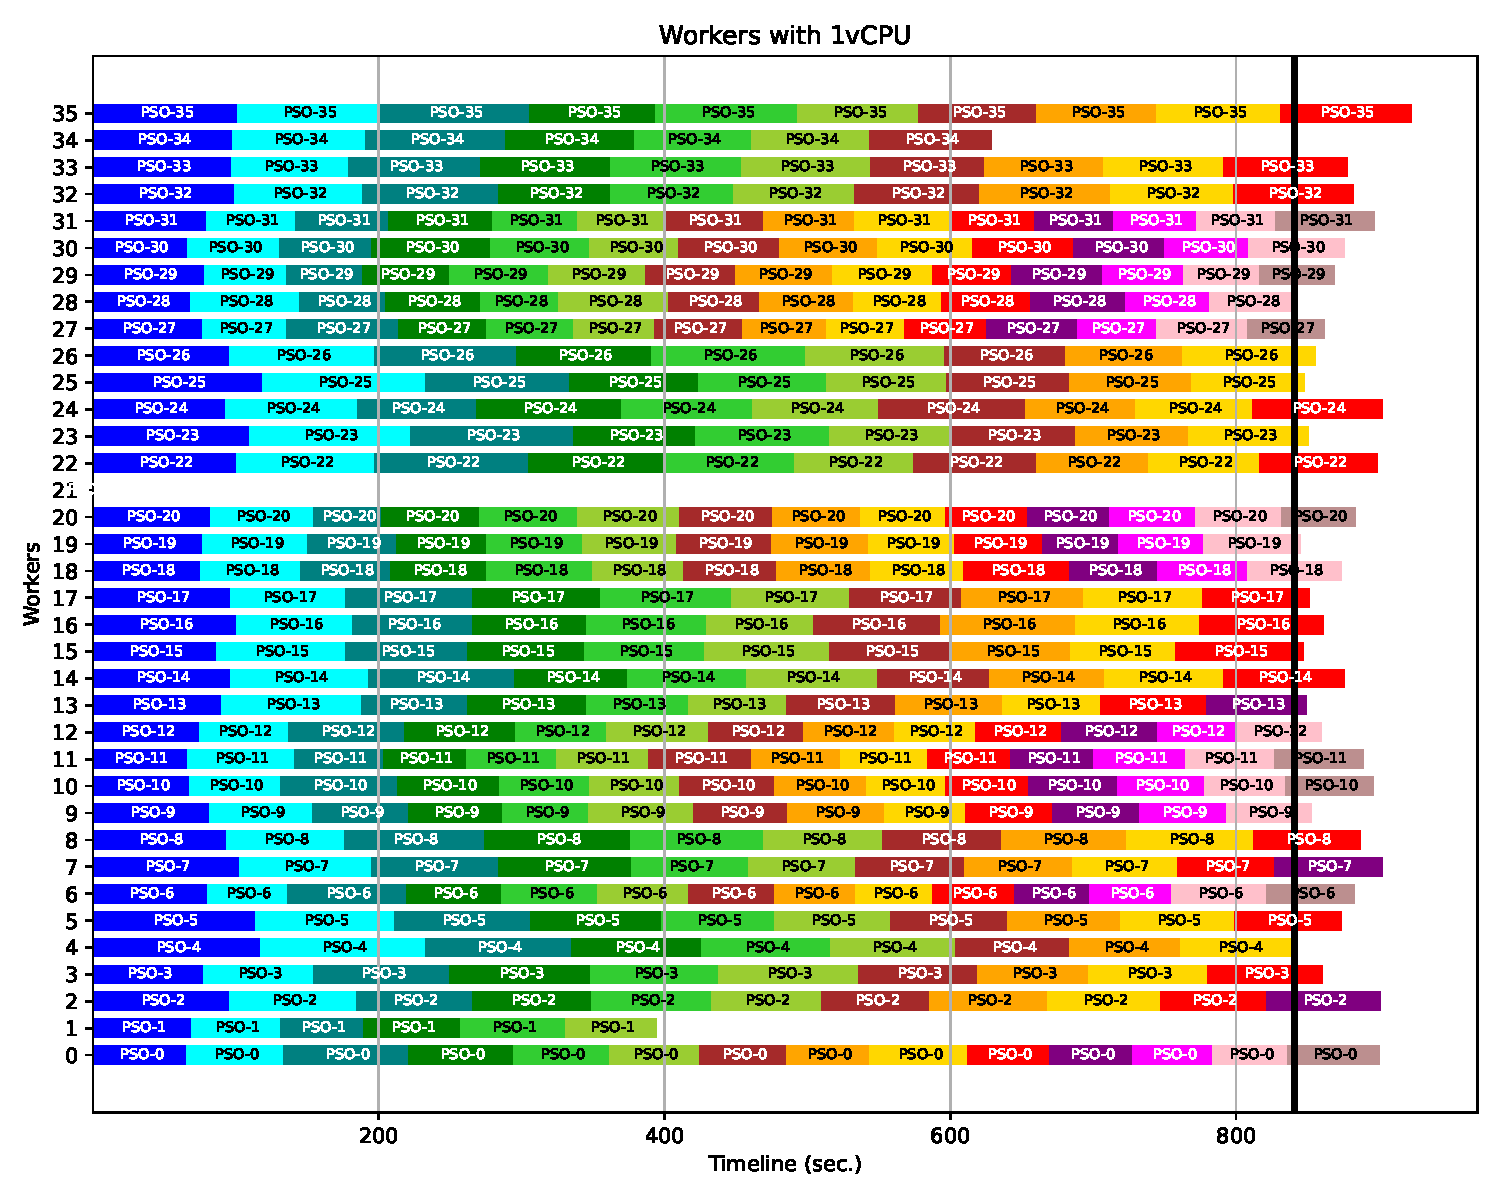
\includegraphics[width=0.8\textwidth]{plotW36P36}
\caption{Execution of 36 workers and 36 swarms, The timeline at the bottom marks 
the progression in seconds, indicating the duration of each PSO instance's activity 
inside a particular worker container.}
\label{fig:36w36s}
\end{figure*}

\section{Cloud-based Deployment}
\label{sec:aws-deployment}


Figure \ref{fig:KafkEO} shows the container-based architecture proposed by García-Valdez and
Merelo \cite{valdez2021container,garcia2018modern} the multi-swarm design. We adapted this initial
design, adding components and strategies that are presented in previous papers. Adapting the 
initial parameters of the algorithm to use an heterogeneous strategy \cite{mancilla2024pendiente} 
together with an adaptation of these parameters considering the diversity and the number of iterations of the algorithm. 
In these previous works we implemented the event-driven design using containers running 
locally in a single workstation. Before explaining in detail the cloud deployment, we first explain the overall design. 
Figure \ref{fig:KafkEO} shows the main components of the system as swim lanes. 
Following an event-driven design, we have two processing components (\texttt{combinator} and \texttt{worker}) that communicate via message queues.  
The data passed and interchanged between components are swarms (or populations) containing 
the current state of the proposed solutions (in these case particles). Decoupling the 
population state from the search algorithm presents several advantages, we can scale 
the system by adding new populations and we can even have multiple algorithms processing 
the populations. In the current implementation we opted for having a single PSO algorithm 
for processing all the populations. This is then a Multi-Swarm PSO.
The \texttt{combinator} process has other responsibilities, but is initially responsible 
for  
the first step. The \texttt{combinator} creates a certain number of swarms, each particle 
is randomly positioned in the search space. Together with the collection of particles the 
initial parameters of the PSO algorithm are also generated. In this case, the parameters 
are randomly generated with in a range of values. This is called a heterogeneous strategy, this strategy 
gives acceptable results without the burden of searching the 
parameters experimentally \cite{mancilla2023optimization}. As a second step (2), the data 
for each swarm is packed in a message in Json format and pushed to the \texttt{input-queue}. 
The queue is constantly consumed by \texttt{Worker Containers}. 
We can have many workers, each worker is a daemon process that takes one message at a 
time from the \texttt{input-queue} (3), reads the PSO parameters contained in the 
message and then runs the specified number of iterations on the received swarm. In 
local PSO algorithm there is not an initialization step, the algorithm takes the 
current state of the swarm, and starts the iteration. After several iterations the 
resulting state of the swarm is pushed to the \texttt{output-queue} (4). The \texttt{combinator} process pulls the resulting swarm 
messages, and checks first if the best solution has been found (5), if this is true the algorithm ends.  
If not, the best solutions are kept in a buffer with the best \emph{k} individuals. 
Then the swarm data is stored in a buffer. If the buffer has a certain number of 
swarms (in this case two) the populations are combined swapping particles between 
the two in a process similar to a one-point crossover (6). This process is similar 
to the migration step of other Multi-swarm PSO algorithms. Before sending the 
modified swarms and depending on the current state of the algorithm a fuzzy 
system adapts the \emph{C1} and \emph{C2} parameters of the swarms and pushes 
the newly generated swarms again to the \texttt{input-queue} starting a new cycle. 

We mentioned earlier that we have several options for the deployment of cloud-native 
application to AWS, the most common approach is to use single or several virtual servers 
using EC2 instances. In our current deployment we opted for using Amazon Elastic Container Service (ECS). 
ECS is a fully-managed container orchestration service, it allows the user to run, 
stop, and manage Docker containers on a cluster, simplifying the process of deploying, managing,
and scaling containerized applications. ECS uses \textit{Task Definitions} as a blueprint for a set of 
containers that run together on the same host. It defines parameters such as which Docker 
images to use, the CPU and memory requirements, networking information, among others.   
A task definition is similar to a \texttt{docker-compose} file in the sense that 
defines the interaction of several containers. To minimize the need to manage the
underlying infrastructure, we use what is called \texttt{Fargate Tasks}, this is a serverless
compute engine that eliminates the need for launching and managing EC2 instances directly. 
We only need to specify the resource requirements needed for our task. 

Figure \ref{fig:aws-deployment}, shows the main cloud computing technologies from 
Amazons AWS we used in the deployment of the multi-swarm algorithm. For each of the
components described previously, we had specified a Docker container definition using 
a \texttt{Docker} file. With this Docker definition we could run the algorithm locally
using a \texttt{docker-compose} script. As a first step for a cloud deployment we need to create 
a repository for each container definition in Amazon Elastic Container Registry (ECR) (1). 
ECR is a fully-managed container registry service provided by AWS. This registry is 
used to store, manage, and deploy Docker container images. The advantage of 
having an image repository is that we can keep several versions of each image. 
As a second step (2), we defined a Fargare Task Definition for each component. We then created a
ECS cluster, an ECS cluster is a logical grouping of container instances or tasks 
on which we can run our containerized applications. We now run the Task Definitions (3),
and observe the logs of the execution in Amazon CloudWatch, this is a monitoring and observability
service. These steps can be realized using a browser-based user interface or 
using command-line interface. 

\begin{figure*}[h]
\centering
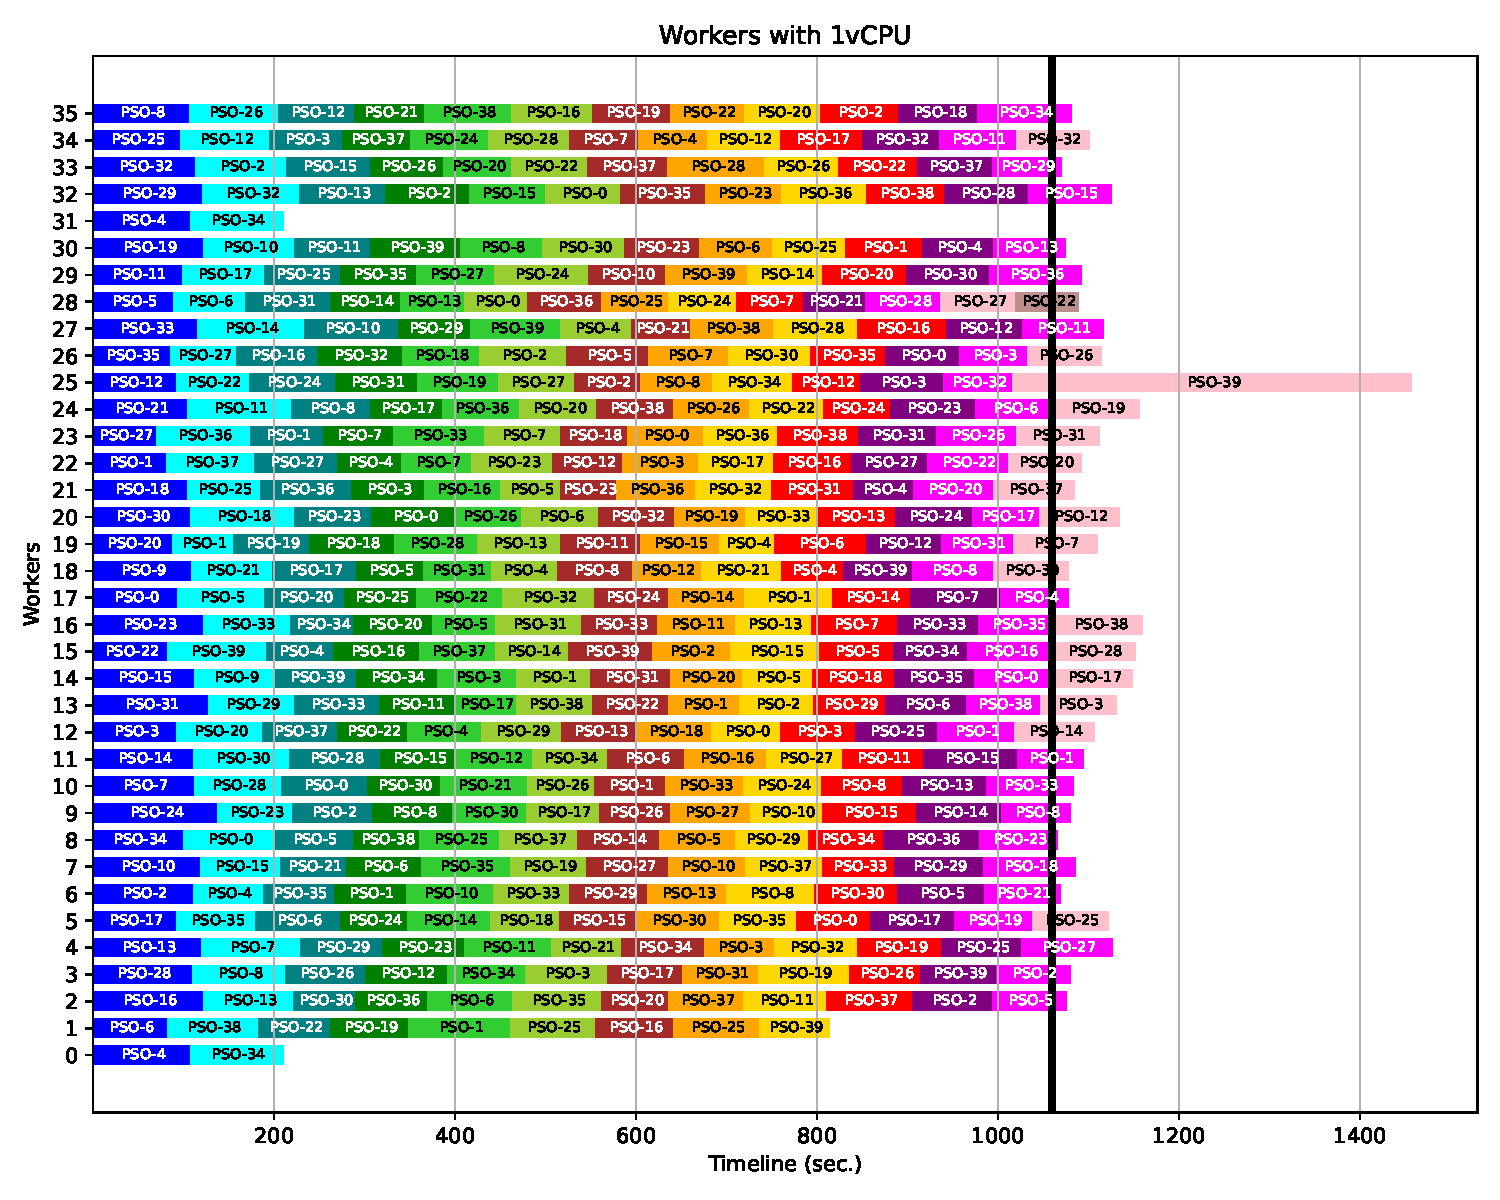
\includegraphics[width=0.8\textwidth]{plotW36P40}
\caption{Execution of 36 workers and 40 swarms. The timeline at the bottom marks 
the progression in seconds, indicating the duration of each PSO instance's activity 
inside a particular worker container.}
\label{fig:36w40s}
\end{figure*}

Each of the services mentioned above has a cost that is charged monthly, the current 
prices are shown in Table \ref{tab:costos}. 
First, we need to consider the cost of storing the Docker container images
in the ECR. We have 50GB a month for free, but is important to remember that
some container images can grow to several GB depending on the 
operating system, languages, libraries, and software included in the container. 
The data transfer cost for a private registry is negligible, there is no cost 
for uploading the images, and there is no data transfer to the outside. 
When we specify the computing resources for running a certain Fargate Task, we
select the number of vCPUs to assign and depending on our selection there
is a minimum and maximum amount of memory we can assign to the task.
At this time, when selecting 1 vCPU the minimum memory is 2 GB and the 
maximum 8 GB, in 1 GB increments. We selected 3 GB memory for our 
containers. For running these experiments, we did not need additional ephemeral storage,
we used the 20 GB included for free. Finally, we used the CloudWatch service extensively,
to keep track of the algorithm and to summarize the results. 

\section{Use Case}
\label{sec:use_case}

To test the deployment we are comparing the time of execution of 
three configurations running on Amazon's Elastic Container Service against 
a local execution using a Mac Studio workstation. We describe next the resource intensive 
optimization problem used as proof-of-concept.

In this case, we want to optimize the membership functions 
for a fuzzy controller for a rear-wheel controller \cite{paden_survey_2016}. 
The fuzzy controller is presented in a previous paper \cite{mancilla2022optimal}.
This problem was selected because it consumes extensive computational resources for
the evaluation of candidate solutions. Figure \ref{fig:Eval} details the evaluation
components for each candidate solution. Each solution consists of a list of real parameters 
for establishing the components of the membership functions for a fuzzy controller definition. 
With this definition we create a controller instance, we then simulate the control
by following several paths with different degrees of difficulty. We then calculate the
average of the RMSEs obtained for each path. This average is considered the fitness of 
the candidate solution. If a controller is not capable of following the track to a certain degree
the simulation is terminated and that controller is assigned the worst fitness value (RMSE=5000).

The current implementation uses the Python language, this means that even if there are 
multiple CPUs in the computer, the Python interpreter process's uses only a 
single thread or CPU at a time. For this reason, we only run workers in 
Fargate instances using a single vCPU. Each vCPU is a hyperthread of an 
Intel Xeon CPU core. We validated this by running a few experiments using 
instances with 4vCPUs but we did not found a substantial difference in the 
compute time, so the additional cost is not justified.

For the cloud configurations we compare use two configurations: 36 and 40 workers. 
This means 36 and 40 vCPUs This number of processors is higher than what we normally
find in a PC Workstation. We are comparing the results with a local implementation 
using a high-end workstation, in this case a 2022 Mac Studio with 
an Apple M1 Ultra chip with 20 CPUs (16 performance and 4 efficiency). We use 16 
workers in this configuration to fully exploit the maximum number of performance cores.

We normally set the number of swarms and the number of workers with a similar value,
if we increase the number of swarms, many will remain in the \texttt{input-queue} waiting 
for a worker to be available. If we have more workers than swarms, the situation is 
worst, because now we will have workers waiting for swarm to be available. 
To test how much the ratio of swarms/workers affects the time of execution we test 
with these three configurations: the same number of swarms and workers with
36 each, 36 workers and 40 swarms, and finally 40 workers and 36 swarms.
 
The multi-swarm is composed of 36 or 40 swarms with ten
particles each, although this is a small size for a traditional 
single swarm PSO, in the case of a MS-PSO the total size of the 
swarm is the sum of all swarms. Each local PSO will run four iterations of the algorithm
before returning the resulting swarm state to the \texttt{output-queue}. All swarms will
complete ten cycles, meaning they will go through the combiner and back to the
\texttt{input-queue} a total of ten times each. 

The parameters of the multi-swarm version of the PSO algorithm are shown in Table 
\ref{tab:alg_params}.
To compare the time-to-solution performance we use as a metric the number of 
function evaluations per second (EPS). As we mentioned before, the fitness 
evaluation function is the most computationally demanding component of the PSO 
algorithm, and this is why the number of calls to this function is a commonly 
used metric to evaluate the amount of work needed to 
find a solution independently of the parameters or hardware used. In this case, 
we change the parameters of the MS-PSO algorithm, depending on the amount 
of swarms and workers available. These changes in the configuration yield 
different numbers of function evaluations for each configuration. To take
this into account, we compare the speed of execution by EPS and higher 
values are better.

\begin{figure*}[h]
\centering
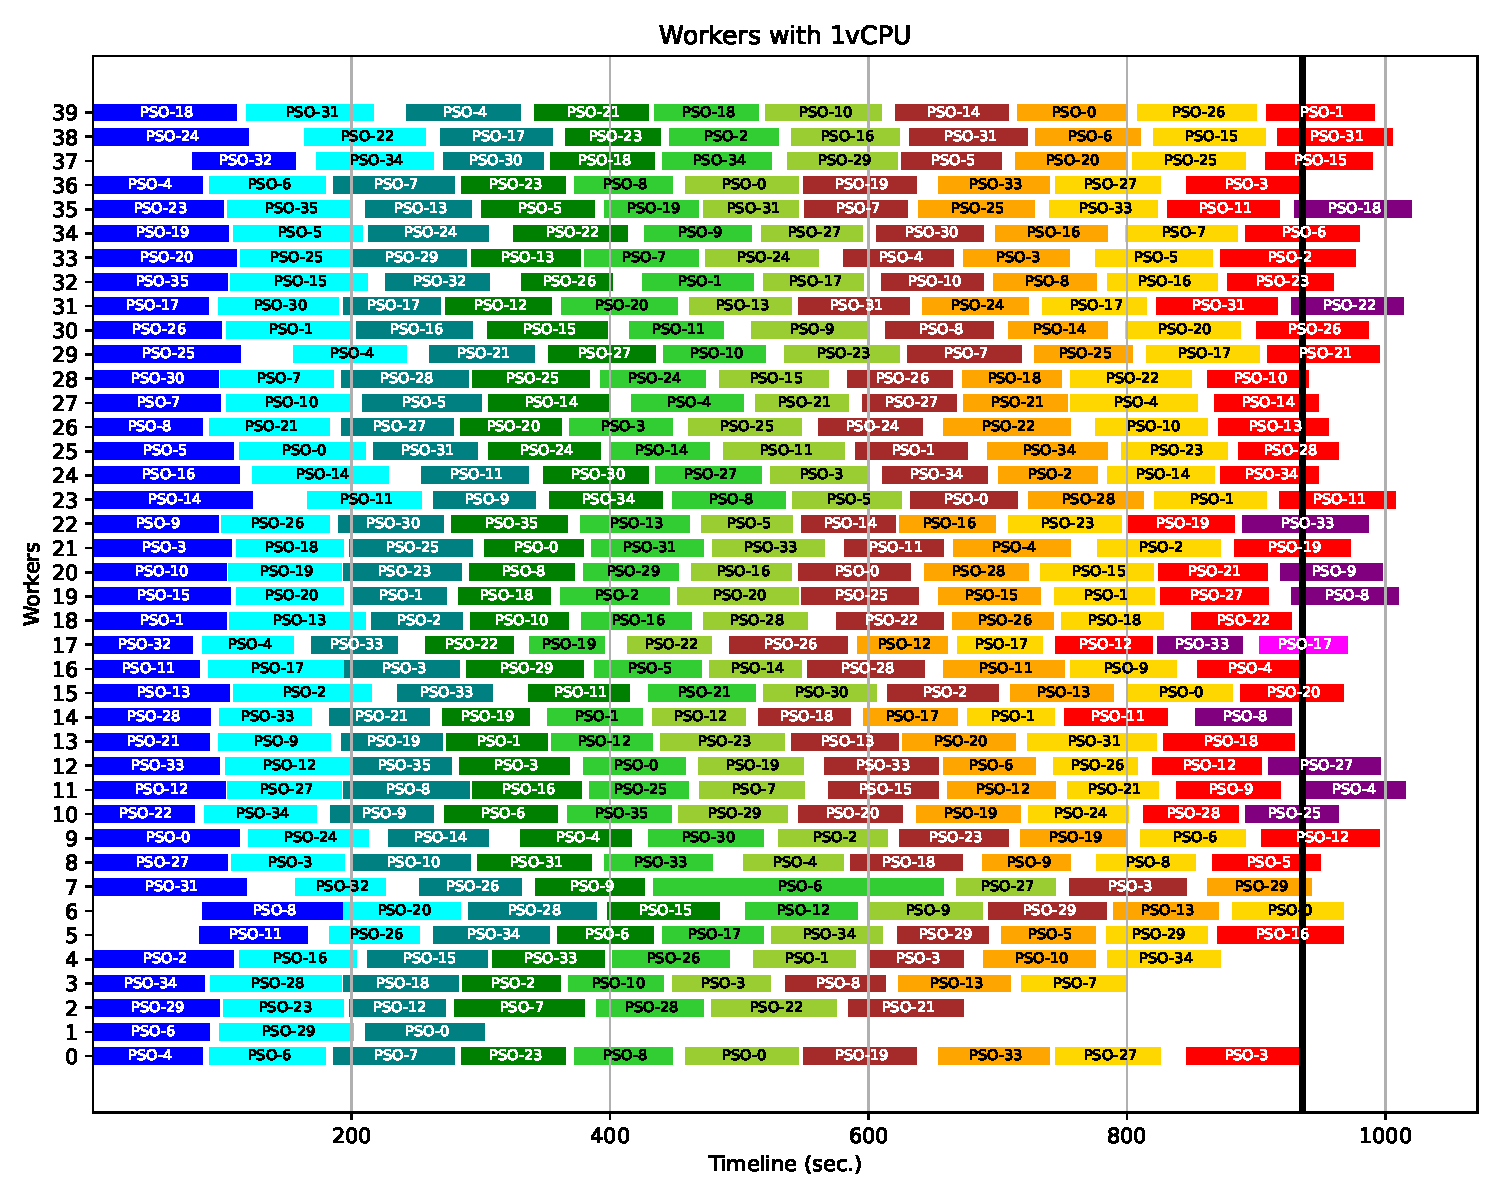
\includegraphics[width=0.8\textwidth]{plotW40P36}
\caption{Execution of 40 workers and 36 swarms.The timeline at the bottom marks 
the progression in seconds, indicating the duration of each PSO instance's activity 
inside a particular worker container.}
\label{fig:40w36s}
\end{figure*}

\section{Results}
\label{sec:results}

Table \ref{tab:aws-results} shows the results for the proposed 
configurations, giving the best RMSE obtained, the total time 
(in seconds) and the function evaluations per second of the experiments.
We also included the cost per execution according to the number of 
workers and the time to finish, considering only the vCPU and Memory costs. 
We can see that there is a significant increase in the \#FE per second when the 
number of swarms is equal to the number of workers. 
These results can be explained by analyzing the timeline of three representative runs. 

First, we describe the format in which the results are presented.
Figures \ref{fig:36w36s} to \ref{fig:40w36s} shows the timelines for the proposed 
configurations. The x-axis shows the time elapsed in seconds from 
the beginning of the experiment. Each row represents a particular worker, identified 
by a sequential number. Each box represents the range of time in seconds, beginning when a
swarm is pulled from the \texttt{input-queue} until is pushed to the \texttt{output-queue}.
Each swarm is identified by a sequential integer. The elapsed time is not the same in 
all cases, because depending on the performance of the controller the time to 
complete the path is different. Also, when the error or distance to 
the path is large the simulation is interrupted thus taking less time.
To identify each swarm, the color corresponds to the order in which it was received 
in each worker, this is to avoid those cases where the same swarm is sequentially received
by the same worker twice. In this case, if the swarm is of the same color it
is difficult to distinguish between the two boxes. The vertical bold line indicates 
the moment in time when the number of evaluations has been reached. At this moment,
no more swarms are pushed to the \texttt{input-queue}. Because workers,
take swarms asynchronously, the work that was already in the \texttt{input-queue} is still 
pulled by workers, and the work they are processing at that time is also finished. 
This is why more work is processed beyond the bold line.

Figure \ref{fig:36w36s} shows the timeline for the experiment using 36 workers and 36 swarms.
When we have this configuration it is very common that each swarm is executed exclusively by 
the same worker. This is because the \texttt{input-queue} will be empty most of the time. Once
a worker finishes the processing of a certain swarm it will be available for
the next swarm in the \texttt{input-queue}. The \texttt{combinator} returns the 
same swarm to the \texttt{initial-queue} and the same worker is available to take
the same swarm again. Furthermore, when this condition happens, there
is not a noticeable waiting time for workers. We can see that this happens in all
the workers. Is important to notice that \emph{worker 21} takes a swarm, but this swarm is 
never pushed back in to the \texttt{output-queue}. This could be because there was 
an error in the swarm configuration or a bug in the code. At this moment, 
we do not have a fault-tolerant solution, for instance, to restart a worker if the work 
is not returned after certain amount of time. But in any case, the nature 
of the event-driven solution still works well in this cases. The extra work needed to 
reach the number of evaluations needed to complete the experiment is 
distributed among all the other workers. Figure \ref{fig:36w40s} show the case 
when we have more swarms than workers, as a consequence, swarms are not always 
processed by the same worker like in the previous case. We need to assess in a 
future work if this behavior is beneficial to the search algorithm. 
The drawback of this case is that the work takes more time because we have 
less resources to do the computation. Finally, Figure \ref{fig:40w36s} shows the 
case in which we have spare workers. The problem with this approach is that 
the workers have to wait until a new population is available, for example 
\emph{worker 5} needs to wait until a
swarm is available. In this case, population PSO-11 is received by \emph{worker 5} 
after \emph{worker 16} finished working on the swarm. Nevertheless, even if we have more computing resources, 
because of the addition idle time of the workers the overall time is not the best. 

When comparing against the local execution, results show that we needed about 2.25 
times the number of workers to match the time-to-finish performance of a local execution.
There are several factors that could have an impact on this difference, the communication time
for a local container network is faster than in a cloud environment, the M1 chip tied with 
a fast memory bandwidth (800GB/s) are faster than a vCPU, there could be differences 
in the virtualization environment in which the docker host runs, the Docker engine used 
in Mac Studio is optimized for the M1 chip. On the other hand, running these type of 
experiments in a cloud environment does not incur in an initial investment on a workstation 
computer. 


\section{Conclusion and Future Work}
\label{sec:conclusionAndFutureWork}

This paper gives details on the cloud-native design and deployment options 
for a multi-swarm PSO algorithm. The algorithm addresses the computationally 
demanding optimization problem of tuning the membership functions
of a fuzzy controller applied on rear-wheel path tracking. We deployed the algorithm 
on Amazon's container platform, and compare this solution against a local 
docker based deployment. We compared the three different configurations to 
highlight the differences between worker and swarm ratios. We found that the 
most effective configuration is to have a configuration with the same number of
workers or threads and swarms. We found that for certain use cases, the 
number of workers needs to be increased when deploying the algorithm to 
a cloud provider. Cloud deployment of cloud-native implementation of 
population-based algorithms is cost effective alternative with out the need of 
investing on additional hardware or administrative costs. 

For future research, we aim to expand upon the design options, on the
algorithmic side and as well as the deployment on the cloud. On the algorithm, we can 
dynamically change the size or number of swarms (and workers) 
to ascertain potential performance gains. When implementing 
these options we can test the auto-scaling features of the cloud platform, 
with the intent to optimize resource utilization with out degrading the
the algorithm's exploratory capacities. 


\section*{Acknowledgements} 
This work is funded by Project 18186.23-P of 2023 TecNM research grants.


% OBLIGATORY: use BIBTEX formatting!
\small{
\bibliographystyle{cys}
\bibliography{biblio}
}
\normalsize


\begin{biography}[]{} % Leave this section empty
\end{biography}

{\vskip 12pt}
\noindent
\footnotesize {\textit{Article received on 06/12/2016; accepted on 16/01/2017.\\
Corresponding author is Mario García-Valdez.}

\end{document}
